\title{On studying neural network expressiveness using topological data analysis and knot theory}

\author{Alexandre Louvet}

\documentclass{article}

\usepackage{graphicx}
\usepackage{tikz}
\usetikzlibrary{decorations.markings}
\usepackage{amsmath}

\usepackage[latin1]{inputenc}
\usepackage{amsfonts}
\usepackage{stmaryrd}

\newfont{\titre}{cmr10 at 11pt}
\newfont{\soustitre}{cmbx10 at 11pt}
\newcommand{\N}{\mathbb{N}}
\newcommand{\Z}{\mathbb{Z}}
\newcommand{\Q}{\mathbb{Q}}
\newcommand{\R}{\mathbb{R}}
\newcommand{\C}{\mathbb{C}}
\newcommand{\U}{\mathbb{U}}
\newcommand{\F}{\mathcal{F}}
\renewcommand{\P}{\mathcal{P}}
\newcommand{\V}{\mathcal{V}}
\renewcommand{\d}{\, \mbox{d}}
\renewcommand{\H}{\mathcal{H}}
\renewcommand{\B}{\mathcal{B}}
\renewcommand{\S}{\mathcal{S}}
\renewcommand{\L}{\mathcal{L}}
\newcommand{\M}{\mathcal{M}}
\newcommand{\GL}{\mbox{GL}}
\renewcommand{\O}{\mbox{O}}
\newcommand{\SO}{\mbox{SO}}
\renewcommand{\Im}{\mbox{Im} \,}
\newcommand{\Tr}{\mbox{Tr} \,}
\newcommand{\rg}{\mbox{rg} \,}
\newcommand{\Id}{\mbox{Id}}
\newcommand{\I}{\mbox{I}}
\newcommand{\sv}{\\[2pt]}
\newcommand{\Sv}{\\[6pt]}
\newcommand{\SV}{\\[9pt]}
\newcommand{\rv}{\\[-6pt]}
\newcommand{\chapitre}{\section*}
\newcommand{\paragraphe}{\subsection*}
\newcommand{\partie}{\subsubsection*}
\newcommand{\debut}{\\[-14pt] \begin{itemize} \parskip -3pt}
\newcommand{\fin}{\end{itemize}}
\let \[ = \llbracket
\let \] = \rrbracket
\def\overcirc #1 {\buildrel \circ \over #1 \ }
\def\bar #1{\hskip1pt\overline{\hskip-1pt#1}\hskip1pt}
\def\interieur #1{{\mathop{#1}\limits^{\circ}}}   % interieur
\def\adherence #1{\hskip1pt\overline{\hskip-1pt#1\hskip1pt}\hskip-1pt} % adherence
\def\modulo #1{\ \left[ #1 \right]}               % modulo
\def\eqv{\mathop{\sim}\limits}                    % equivalence
\def\vct#1{\hskip1pt\overrightarrow{\hskip-1pt#1\hskip1pt}\hskip-1pt} % vecteur
\def\rac#1#2{\root {\scriptstyle #1} \of {#2}}    % racine
\def\dcap {\bigcap\limits}            % intersection
\def\dcup {\bigcup\limits}            % union
\def\dlim  {\lim\limits}              % limite (lim)
\def\dprod {\prod\limits}             % produit
\def\dsum  {\sum\limits}              % somme
\def\dint  {\displaystyle\int}        % integrale

\parindent = 0mm


\newtheorem{theorem}{Theorem}
\newtheorem{lemma}{Lemma}
\newtheorem{proposition}{Proposition}
\newtheorem{scolium}{Scolium} 
\newtheorem{definition}{Definition}
\newenvironment{proof}{{\sc Proof:}}{\hfill $\square$}
\newenvironment{AMS}{}{}
\newenvironment{keywords}{}{}

\def\layersep{2.5cm}

\begin{document}
\newpage
\maketitle
\begin{abstract}
  In this paper we summarize the state of the art on the question of neural network expressiveness both on the theoretical approach to the problem with the study of universal approximators and some practical approaches using topological data analysis and trajectories. We then propose an analysis of the question from a knot theory perspective and share results using studied methods for datasets in dimension 3 and 4.
\end{abstract}

\newpage

\tableofcontents

\newpage

\section{Neural network expressiveness}

\subsection{Definition}

Let $I_n$ denote the $n$-dimensional unit cube $[0,1]^n$ and $\F(I_n,\R)$ be the space of functions from $I_n$ to $\R$. We want to study the density of the subsets $S_f$ of $\F(I_n,\R)$ that can be written as follows:\\

\begin{center}
  $S_f = \{G_N(x) \in \F(I_n,\R) \mid G(x) = \sum\limits_{i=1}^{N} \alpha_i f(y_j^T x + \theta_j )\}$, $N \in \N $
\end{center}

depending on the choice of $f \in \F(\R,\R)$. In the previous equation $y_j \in \R^n$ and $\alpha_j, \theta \in \R$, $y^T$ is the transpose of y and $y^Tx$ is the inner product of $y$ and $x$.\\

The study of neural network expressiveness consists of the problem described above when $f$ is a function used as an activation function for neural network. The study of density can be on the whole set $\F(I_n,\R)$ or on subsets of it such as $\C(I_n,\R)$ the set of continuous functions from $I_n$ to $\R$.\\

In particular if $S_f$ is dense in a subset $A \subseteq \F(I_n, \R)$ we will say that a single-layer feed-forward neural network (Fig. 1) with $f$ as its activation function is a \textit{universal approximator} of $A$. Considering a neural network has a finite number of nodes neural network expressiveness also consists of the study of the rate of approach of the approximation, i.e. the sudy of \\

\begin{center}
  $\lim\limits_{N \to \infty} H(N) = \max\limits_{h\in A} (\min\limits_{G_n \in S_f} (\parallel G_n - h \parallel))$ with $\parallel . \parallel$ the cannonical norm on $\F(I_n, \R)$
\end{center}

The study of that limit and especially of its asympatotic approximation gives an idea of the efficiency of the approximator, i.e. the amount of node to add to the network to improve the approximation.\\

\begin{center}
  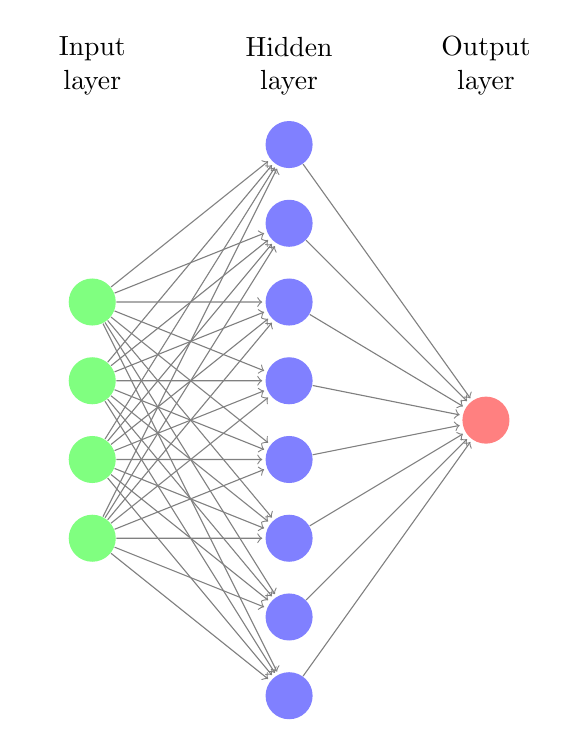
\begin{tikzpicture}[shorten >=1pt,->,draw=black!50, node distance=\layersep]
      \tikzstyle{every pin edge}=[<-,shorten <=1pt]
      \tikzstyle{neuron}=[circle,fill=black!25,minimum size=17pt,inner sep=0pt]
      \tikzstyle{input neuron}=[neuron, fill=green!50];
      \tikzstyle{output neuron}=[neuron, fill=red!50];
      \tikzstyle{hidden neuron}=[neuron, fill=blue!50];
      \tikzstyle{annot} = [text width=4em, text centered]

      % Draw the input layer nodes
      \foreach \name / \y in {1,...,4}
      % This is the same as writing \foreach \name / \y in {1/1,2/2,3/3,4/4}
      \node[input neuron] (I-\name) at (0,-\y) {};

      % Draw the hidden layer nodes
      \foreach \name / \y in {1,...,8}
          \path[yshift=2.0cm]
              node[hidden neuron] (H-\name) at (\layersep,-\y cm) {};

      % Draw the output layer node
      \node[output neuron, right of=H-5,yshift=0.5cm] (O) {};

      % Connect every node in the input layer with every node in the
      % hidden layer.
      \foreach \source in {1,...,4}
          \foreach \dest in {1,...,8}
              \path (I-\source) edge (H-\dest);

      % Connect every node in the hidden layer with the output layer
      \foreach \source in {1,...,8}
          \path (H-\source) edge (O);

      % Annotate the layers
      \node[annot,above of=H-1, node distance=1cm] (hl) {Hidden layer};
      \node[annot,left of=hl] {Input layer};
      \node[annot,right of=hl] {Output layer};
  \end{tikzpicture}\\
Fig 1: A single-layer feed-forward neural network with $n=4$ and $N=8$
\end{center}

\subsection{Universal Approximator}

In this section we will study the different subsets on which the logistic and ReLU functions acts as universal approximators.\\ 

\subsubsection{Sigmoidal functions}

We say that a function $\sigma \in \F(I_n, \R)$ is a sigmoidal function if:\\

\begin{center}
  $\sigma(x) \to
  \begin{cases}
    0 &\text{as $t \to +\infty$}\\
    1 &\text{as $t \to -\infty$}
  \end{cases}$
\end{center}

The sigmoidal functions include the logistic function defined as:\\

\begin{center}
  $f(x) = \frac{1}{1+e^{-x}}$
\end{center}

widely used as an activation function for neural networks.\\

The first study of neural network expressiveness with sigmoidal functions date back to by G.Cybenko in 1989 \cite{cybenko_approximation_1989}. He proves that $S_\sigma$ for $\sigma$ a sigmoidal function is dense in regards of the supremum norm in $C(I_n, \R)$. The demonstration goes as follows.\\

We denote $M(I_n)$ the space of signed regular Borel measures on $I_n$\\

\begin{definition}
  $\sigma$ \text{is discriminatory if} $\mu \in M(I_n)$ \text{and}\\ 
  \begin{center}
  $\forall y \in \R^n,$ $\theta \in \R \int\limits_{I_n} \sigma(y^Tx + \theta) d\mu(x) = 0 \implies \mu = 0$
\end{center}
\end{definition}

\begin{theorem}
  Let $\sigma$ be a contininuous discriminatory function. Then finite sums of the form\\\begin{center}
    $G(x) = \sum\limits_{i=1}^N \alpha_i \sigma(y^Tx + \theta_i)$
  \end{center}
  are dense in $C(I_n, \R)$
\end{theorem}

\begin{proof}
  Let $S \subset C(I_n)$ be the set of the function of the form $G(x)$. S in a linear subset of $C(I_n)$. Let us show that the closure of $S$ is $C(I_n)$.\\
  Assume it is not the case. Then the closure of $S$, denoted $R$, is a proper subspace of $C(I_n)$. Using the Hahn-Banach theorem, there esists $L$ a bounded linear functional on $C(I_n)$ with $L \ne 0$ and  $L(R) = L(S) = 0$\\
  Using the Riesz Representation Theorem, we obtain:\\
  \begin{center}
    $L(h) = \int\limits_{I_n} h(x)d\mu(x)$
  \end{center}
  for some $\mu \in M(I_n)$, for all $h\in C(I_n)$. Since $\sigma(y^Tx + \theta_i)  \in R$, we have\\
  \begin{center}
    $\forall y, \theta \int\limits_{I_n} \sigma(y^Tx + \theta) d\mu(x) = 0$
  \end{center}
  Since $\sigma$ is discriminatory, we have $\mu = 0$ and $L = 0$ follows!
  Hence the closure of $S$ is $C(I_n)$ and by definition $S$ is dense in $C(I_n)$
\end{proof}\\
\Sv
  Now let us show that sigmoidal functions are discriminatory.
  \begin{lemma}
    Any bounded, measurable sigmoidal function, a, is discriminatory. In particular, any continuous sigmoidal function is discriminatory.
  \end{lemma}

  \begin{proof}
    First note $\forall x,y,\theta, \phi$ 
\begin{center}
  $\sigma_\lambda(x) = \sigma(\lambda (y^Tx + \theta) + \phi)
  \begin{cases}
    \to 1 &\text{for $y^Tx+\theta > 0$ as $\lambda \to +\infty$}\\
    \to 0 &\text{for $y^Tx+\theta < 0$ as $\lambda \to +\infty$}\\
    =\sigma(\phi) & \text{for $y^Tx+\theta = 0$}
  \end{cases}$
\end{center}
Thus $\sigma_\lambda(x)$ converges pointwise and boundedly to:

\begin{center}
  $\gamma(x)
  \begin{cases}
    =1 &\text{for $y^Tx+\theta > 0$}\\
    =0 &\text{for $y^Tx+\theta < 0$}\\
    =\sigma(\phi) & \text{for $y^Tx+\theta = 0$}
  \end{cases}$
\end{center}
as $\lambda \to +\infty$\\
\sv
Let $\Pi_{y,\theta} = \{x \mid y^Tx+\theta = 0\}$ and let $H_{y,\theta} = \{x \mid y^Tx + \theta > 0\}$. Lesbegue bounded convergence theorem gives us:\\
\begin{center}
  $0 = \int\limits_{I_n}\sigma_\lambda(x)d\mu(x)$\\
  $ = \int\limits_{I_n} \gamma(x)d\mu(x)$\\
  $\sigma(\phi)\mu(\Pi_{y,\theta}) + \mu(H_{y,\theta})$
\end{center}
for all $\phi, \theta, y$\\
\sv
Fix $y$, we write \\
\begin{center}
  $F(h) = \int_{I_n}h(y^Tx)d\mu(x)$
\end{center}
Note that $F$ is a bounded function on $L^\infty(\R)$ since $\mu$ is a signed mesure. By chosing  $h$ as the indicator function on $[\theta, \infty[$, we have:
\begin{center}
  $F(h) = \int_{I_n} h(y^Tx) d\mu(x) = \mu(\Pi_{y,-\theta}) + \mu(H_{y,-\theta}) = 0$
\end{center}
By linearity $F(h) = 0$ for indicator function on any interval and hence for any simple function (sum of indicator functions) and since simple functions are dense in $L^{\infty}(\R), F = 0$.
In particular it is true for the bounded function $s(u) = sin(m.u)$ and $c(u) = cos(m.u)$. It gives:
\begin{center}
  $F(s+ic) = \int_{I_n} cos(m^Tx) + i sin(m^Tx) d\mu(x) = \int_{I_n} exp(im^Tx)d\mu(x) = 0$
\end{center}
for all $m$. Therefore the fourier transform of $\mu$ is 0 and $\mu$ must be 0. Hence $\sigma$ is discriminatory.
  \end{proof}\\

  This proves that any function of $C(I_n, \R)$ can be approximated by a single-layer network with sigmoidal functions as activation function.\\

  In 1991, Hornik extended in \cite{hornik_approximation_1991} gave the proof for bounded non-constant functions of $F(I_n,\R)$. The proof is very similar to the original one.\\

\subsubsection{ReLU functions}

ReLU functions stands for Rectified Linear Units, there are formed of two pieces of linear functions. They gained interest recently by showing convincing results in a lot of different applications.\\ 

In 2016 Arora et al. \cite{arora_understanding_2018} showed a version of the universal approximation theorem for piecewise linear function that includes ReLU functions.\\

\begin{definition}
  We say a function $f: \R^n \to \R$ is continuous piecewise linear (PWL) if there exists a finite set of polyhedra whose union is $\R^n$, and $f$ is affine linear over each polyhedron (implies continuity because affine regions are closed and cover $\R^n$)
\end{definition}

\begin{proposition}
  Every function in $L^q(\R^n), (1 \le q \le \infty)$ can be arbitrarily approximated in the $L^q$ norm (which for a function $f$ is given by $||f||_q = (\int |f|^q)^{1/q}$) by a ReLU Deep Neural Network.
\end{proposition}

\begin{proof}

  We know that any ReLU DNN represents a PWL function, let's prove the converse.\\
  \sv
  By theorem 1 in \cite{wang_generalization_2005} any piecewise linear function $f: \R^n \to \R$, can be written:\\
  \begin{center}
    $f = \sum\limits_{j=1}^{p}s_j(\max\limits_{i\in S_j} l_i)$
  \end{center}
  with $l_i$ $(i\le i \le k)$ linear functions, $S_i$ $(1 \le i \le p) \subseteq \{1, ..., k\}$ with $\forall i, |S_i| \le n + 1$ and $\forall j \in \{1,...,p\},  s_j \in \{-1, +1\}$ \\
  \sv
  It means that any PWL convex function can be represented as a linear combination of at most $n+1$ affine pieces. That's to say a ReLU DNN with size $n+1$.\\
  \SV
  Let $p \in \N^*$, let $f \in L^p(\R^n)$, consider the function sequence:\\
  \begin{center}
    $f_n(x) = (x - \frac{k}{n})f(\frac{k}{n}) + (1 - x + \frac{k}{n})f(\frac{k+1}{n})$ with $\frac{k}{n} \le x < \frac{k+1}{n}, n \ge 1$ 
  \end{center}

  $f_n \xrightarrow[n \to \infty]{} f$, and $\forall n, f_n$ is a PWL continous function. Therefore the continuous PWL functions are dense in $L^p(\R^n)$.
  \SV
  Since any PWL function $\R^n \to \R$ is representable by a ReLU DNN, unniversal approximation theorem follows from the fact that the family of continuous PWL functions is dense in any $L^p(\R^n)$ space for $1 \le p \le \infty$. 
  
\end{proof}\\
\SV
In this article, Arora et al. also give a higher bound for the depth of the network. they show that the network required for any function $f \in L^q(\R^n)$ is at most $\lceil log_2(n+1) \rceil$.\\

In 2018, Hannin \& Selke \cite{hanin_approximating_2018} showed that the minimal width a ReLUneural network must have in order to approximate any function $f: \R^n \to \R^m$ is $n + m$. Giving a lower bound to the width of the ReLU network.

\section{Homology}

The study of homology is part of the field of algebraic topology. We will first introduce the concept of homology, then take a look at the theoretical concept behind it by introducing $\Delta$-complex: a primitive topolgical structure that allow the study of homology. Then with the introduction of simplicial homology and finally singular homology we will complete the presentation of the fundamental objects used in the study of homolgy. We will then reconsider these tools in the context of our research. This part heavily relies on the book \textit{Algebraic Topolgy} by A. Hatcher \cite{hatcher_algebraic_2002} and the class given by P. Albin at University of Illinois \cite{albin_1_2018} with the same book as class material. 

\subsection{The idea of homology}

\begin{center}
  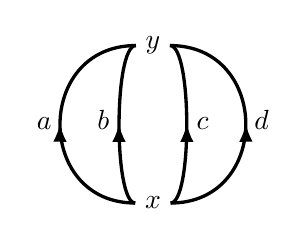
\begin{tikzpicture}[node distance={20mm}] 
    \node[draw=none] (1) {$x$}; 
    \node[draw=none] (2) [above of=1] {$y$}; 
    %\node at (1)[circle,fill,inner sep=1pt]{}
    %\node at (2)[circle,fill,inner sep=1pt]{}
\begin{scope}[very thick,decoration={
    markings,
    mark=at position 0.5 with {\arrow{latex}}}
    ] 
    \draw[postaction={decorate}] (1) .. controls +(left:1.5cm) and +(left:1.5cm) .. (2)
\foreach \p in {$a$} {node[sloped,above,pos=0.5,rotate=-90, xshift=-0.2cm, yshift=-0.2cm]{\p}};
 \draw[postaction={decorate}] (1) .. controls +(left:0.5cm) and +(left:0.5cm) .. (2)
\foreach \p in {$b$} {node[sloped,above,pos=0.5,rotate=-90, xshift=-0.2cm, yshift=-0.2cm]{\p}};
 \draw[postaction={decorate}] (1) .. controls +(right:0.5cm) and +(right:0.5cm) .. (2)
\foreach \p in {$c$} {node[sloped,above,pos=0.5,rotate=90, xshift=0.2cm, yshift=-0.2cm]{\p}};
 \draw[postaction={decorate}] (1) .. controls +(right:1.5cm) and +(right:1.5cm) .. (2)
\foreach \p in {$d$} {node[sloped,above,pos=0.5,rotate=90, xshift=0.2cm, yshift=-0.2cm]{\p}};
\end{scope}
\end{tikzpicture} 
\end{center}

Consider the figure drawn above. We can see two points $x$ and $y$ as well as four edges $a$, $b$, $c$ and $d$. Consider the loops formed by travelling along the edges, for instance the path $ab^{-1}$ is a loop with $x$ as the basepoint. Something to consider is that the loop $b^{-1}a$ is basically the same loop but starting from a different basepoint, $y$ in that case. By abelianizing the process, we can consider cycles instead of loops without any basepoint.\\

The abelian groups having only one operation, we will then switch to additive notations to remain in accordance with Hatcher's notations. With that new notation we can write equalities such as $(a-c) + (b-d) = (a-d) + (b-c)$. This is justified by the fact that from an algebraic point of view, there is no difference between these two cycles.\\

Let us call any linear combination of edges, chains. Then the condition for a chain $ka + lb + mc + nd$ with $k,l,m,n \in \N$ to be a cycle is $k + l + m + n = 0$.\\



\subsection{$\Delta$-complexes}

\subsection{Simplical homology}

\subsection{Singular homology}

\subsection{Homology in our research}

Homology exists as a computable alternative homotopy.

\section{Topological data Analysis}

\subsection{Fundamental concepts}

\subsection{Persistent homology}

\section{Knot theory}

\subsection{Definition}

\subsection{Knot determinant}

\subsubsection{Definition}

\subsubsection{Algorithms}

\section{Measuring neural network expressiveness}

\subsection{Using topological data analysis}

\subsection{Using trajectories}

\section{The study of trajectories from a knot theory perspective}

\subsection{Methodology}

\subsection{Algorithms}

\subsection{Results}

\section{Extending the study of expressiveness with topological data analysis} 
\subsection{Methodology}

\subsection{Algorithms}

\subsection{Results}

\newpage

\bibliography{bibliography}

\bibliographystyle{ieeetr}

\end{document}

